\documentclass[]{article}
\usepackage{lmodern}
\usepackage{amssymb,amsmath}
\usepackage{ifxetex,ifluatex}
\usepackage{fixltx2e} % provides \textsubscript
\ifnum 0\ifxetex 1\fi\ifluatex 1\fi=0 % if pdftex
  \usepackage[T1]{fontenc}
  \usepackage[utf8]{inputenc}
\else % if luatex or xelatex
  \ifxetex
    \usepackage{mathspec}
  \else
    \usepackage{fontspec}
  \fi
  \defaultfontfeatures{Ligatures=TeX,Scale=MatchLowercase}
\fi
% use upquote if available, for straight quotes in verbatim environments
\IfFileExists{upquote.sty}{\usepackage{upquote}}{}
% use microtype if available
\IfFileExists{microtype.sty}{%
\usepackage{microtype}
\UseMicrotypeSet[protrusion]{basicmath} % disable protrusion for tt fonts
}{}
\usepackage[margin=1in]{geometry}
\usepackage{hyperref}
\hypersetup{unicode=true,
            pdftitle={Crime in Chicago: A Data Analysis Summary using R},
            pdfauthor={Student ID: 201081646},
            pdfborder={0 0 0},
            breaklinks=true}
\urlstyle{same}  % don't use monospace font for urls
\usepackage{color}
\usepackage{fancyvrb}
\newcommand{\VerbBar}{|}
\newcommand{\VERB}{\Verb[commandchars=\\\{\}]}
\DefineVerbatimEnvironment{Highlighting}{Verbatim}{commandchars=\\\{\}}
% Add ',fontsize=\small' for more characters per line
\usepackage{framed}
\definecolor{shadecolor}{RGB}{248,248,248}
\newenvironment{Shaded}{\begin{snugshade}}{\end{snugshade}}
\newcommand{\KeywordTok}[1]{\textcolor[rgb]{0.13,0.29,0.53}{\textbf{{#1}}}}
\newcommand{\DataTypeTok}[1]{\textcolor[rgb]{0.13,0.29,0.53}{{#1}}}
\newcommand{\DecValTok}[1]{\textcolor[rgb]{0.00,0.00,0.81}{{#1}}}
\newcommand{\BaseNTok}[1]{\textcolor[rgb]{0.00,0.00,0.81}{{#1}}}
\newcommand{\FloatTok}[1]{\textcolor[rgb]{0.00,0.00,0.81}{{#1}}}
\newcommand{\ConstantTok}[1]{\textcolor[rgb]{0.00,0.00,0.00}{{#1}}}
\newcommand{\CharTok}[1]{\textcolor[rgb]{0.31,0.60,0.02}{{#1}}}
\newcommand{\SpecialCharTok}[1]{\textcolor[rgb]{0.00,0.00,0.00}{{#1}}}
\newcommand{\StringTok}[1]{\textcolor[rgb]{0.31,0.60,0.02}{{#1}}}
\newcommand{\VerbatimStringTok}[1]{\textcolor[rgb]{0.31,0.60,0.02}{{#1}}}
\newcommand{\SpecialStringTok}[1]{\textcolor[rgb]{0.31,0.60,0.02}{{#1}}}
\newcommand{\ImportTok}[1]{{#1}}
\newcommand{\CommentTok}[1]{\textcolor[rgb]{0.56,0.35,0.01}{\textit{{#1}}}}
\newcommand{\DocumentationTok}[1]{\textcolor[rgb]{0.56,0.35,0.01}{\textbf{\textit{{#1}}}}}
\newcommand{\AnnotationTok}[1]{\textcolor[rgb]{0.56,0.35,0.01}{\textbf{\textit{{#1}}}}}
\newcommand{\CommentVarTok}[1]{\textcolor[rgb]{0.56,0.35,0.01}{\textbf{\textit{{#1}}}}}
\newcommand{\OtherTok}[1]{\textcolor[rgb]{0.56,0.35,0.01}{{#1}}}
\newcommand{\FunctionTok}[1]{\textcolor[rgb]{0.00,0.00,0.00}{{#1}}}
\newcommand{\VariableTok}[1]{\textcolor[rgb]{0.00,0.00,0.00}{{#1}}}
\newcommand{\ControlFlowTok}[1]{\textcolor[rgb]{0.13,0.29,0.53}{\textbf{{#1}}}}
\newcommand{\OperatorTok}[1]{\textcolor[rgb]{0.81,0.36,0.00}{\textbf{{#1}}}}
\newcommand{\BuiltInTok}[1]{{#1}}
\newcommand{\ExtensionTok}[1]{{#1}}
\newcommand{\PreprocessorTok}[1]{\textcolor[rgb]{0.56,0.35,0.01}{\textit{{#1}}}}
\newcommand{\AttributeTok}[1]{\textcolor[rgb]{0.77,0.63,0.00}{{#1}}}
\newcommand{\RegionMarkerTok}[1]{{#1}}
\newcommand{\InformationTok}[1]{\textcolor[rgb]{0.56,0.35,0.01}{\textbf{\textit{{#1}}}}}
\newcommand{\WarningTok}[1]{\textcolor[rgb]{0.56,0.35,0.01}{\textbf{\textit{{#1}}}}}
\newcommand{\AlertTok}[1]{\textcolor[rgb]{0.94,0.16,0.16}{{#1}}}
\newcommand{\ErrorTok}[1]{\textcolor[rgb]{0.64,0.00,0.00}{\textbf{{#1}}}}
\newcommand{\NormalTok}[1]{{#1}}
\usepackage{graphicx,grffile}
\makeatletter
\def\maxwidth{\ifdim\Gin@nat@width>\linewidth\linewidth\else\Gin@nat@width\fi}
\def\maxheight{\ifdim\Gin@nat@height>\textheight\textheight\else\Gin@nat@height\fi}
\makeatother
% Scale images if necessary, so that they will not overflow the page
% margins by default, and it is still possible to overwrite the defaults
% using explicit options in \includegraphics[width, height, ...]{}
\setkeys{Gin}{width=\maxwidth,height=\maxheight,keepaspectratio}
\IfFileExists{parskip.sty}{%
\usepackage{parskip}
}{% else
\setlength{\parindent}{0pt}
\setlength{\parskip}{6pt plus 2pt minus 1pt}
}
\setlength{\emergencystretch}{3em}  % prevent overfull lines
\providecommand{\tightlist}{%
  \setlength{\itemsep}{0pt}\setlength{\parskip}{0pt}}
\setcounter{secnumdepth}{5}
% Redefines (sub)paragraphs to behave more like sections
\ifx\paragraph\undefined\else
\let\oldparagraph\paragraph
\renewcommand{\paragraph}[1]{\oldparagraph{#1}\mbox{}}
\fi
\ifx\subparagraph\undefined\else
\let\oldsubparagraph\subparagraph
\renewcommand{\subparagraph}[1]{\oldsubparagraph{#1}\mbox{}}
\fi

%%% Use protect on footnotes to avoid problems with footnotes in titles
\let\rmarkdownfootnote\footnote%
\def\footnote{\protect\rmarkdownfootnote}

%%% Change title format to be more compact
\usepackage{titling}

% Create subtitle command for use in maketitle
\newcommand{\subtitle}[1]{
  \posttitle{
    \begin{center}\large#1\end{center}
    }
}

\setlength{\droptitle}{-2em}

  \title{Crime in Chicago: A Data Analysis Summary using R}
    \pretitle{\vspace{\droptitle}\centering\huge}
  \posttitle{\par}
    \author{Student ID: 201081646}
    \preauthor{\centering\large\emph}
  \postauthor{\par}
    \date{}
    \predate{}\postdate{}
  
\usepackage{float} \floatplacement{figure}{H}

\begin{document}
\maketitle

\section{Introduction}\label{introduction}

This report is the first assessment of the \textbf{MATH5741M Statistical
Theory and Methods} module. Its aims are to summarise a crime dataset
from the city of Chicago and answer the following research questions:

\begin{itemize}
\item
  How has crime evolved over time in the city of Chicago?
\item
  What time of day do most crime occur?
\item
  In which locations of the city is crime more likely to happen?
\item
  Which districts are more potentially dangerous?
\end{itemize}

\section{Data and methods}\label{data-and-methods}

The analysis is done with a sample of the
\href{https://data.cityofchicago.org/Public-Safety/Crimes-2001-to-present/ijzp-q8t2}{crime
dataset from the Chicago Police Department} which contains all the crime
incidents that occurred in the city of Chicago from 2001 to the present.

We first prepare the data, creating, transforming and cleaning the
variables we are interested in. Then, we perform the statistical
analysis through line graphs, bar graphs and heat-maps which will answer
each of our research questions.

The report has been done with \texttt{Rmarkdown} and it is code
reproducible. However, due to space limitation (it should not be more
than 6 pages in total) does not include all the code written for its
performance. \footnote{To see the whole code visit
  \url{https://github.com/eugenividal/Chicago-Crime-Data-Analysis}.}

\section{Results}\label{results}

\subsection{Data preparation}\label{data-preparation}

First, we activate the libraries we will need to set up the project.

\begin{Shaded}
\begin{Highlighting}[]
\CommentTok{# Activate libraries}
\KeywordTok{library}\NormalTok{(ggplot2)}
\KeywordTok{library}\NormalTok{(lubridate)}
\KeywordTok{library}\NormalTok{(zoo)}
\KeywordTok{library}\NormalTok{(dplyr)}
\KeywordTok{library}\NormalTok{(knitr)}
\end{Highlighting}
\end{Shaded}

Second, we load the data into the \texttt{R} environment.

\begin{Shaded}
\begin{Highlighting}[]
\CommentTok{# Read csv in R}
\NormalTok{dd=}\KeywordTok{read.csv}\NormalTok{(}\StringTok{"http://www1.maths.leeds.ac.uk/~charles/math5741/crime.csv"}\NormalTok{,}\DataTypeTok{header=}\NormalTok{T)}
\end{Highlighting}
\end{Shaded}

\pagebreak

Third, we create two new variables \texttt{Count} and \texttt{Hour} and
make some necessary transformations in date variables in order to make
\texttt{R} understand them.

\begin{Shaded}
\begin{Highlighting}[]
\CommentTok{# Create a variable count with value 1}
\NormalTok{dd$Count <-}\StringTok{ }\DecValTok{1}
\CommentTok{# Convert Date from factor to date}
\NormalTok{dd$Date <-}\StringTok{ }\KeywordTok{mdy_hms}\NormalTok{(dd$Date)}
\CommentTok{# Extract hour from Date}
\NormalTok{dd$Hour <-}\StringTok{ }\KeywordTok{substring}\NormalTok{(dd$Date, }\DecValTok{12}\NormalTok{,}\DecValTok{13}\NormalTok{)}
\CommentTok{# Drop time from Date}
\NormalTok{dd$Date <-}\StringTok{ }\KeywordTok{as.Date}\NormalTok{(dd$Date, }\DataTypeTok{format=}\StringTok{"%m/%d/%Y"}\NormalTok{)}
\end{Highlighting}
\end{Shaded}

Fourth, we group in larger categories the existent ones in the variables
\texttt{Primary.Type} and \texttt{Location.Description}, and call them
\texttt{Type\_grouped} and \texttt{Location\_grouped}
respectively\footnote{The code written to group the variables'
  categories can be seen at
  \url{https://github.com/eugenividal/Chicago-Crime-Data-Analysis}}.

The next step is to drop all those columns we do not need to answer our
research questions.

\begin{Shaded}
\begin{Highlighting}[]
\CommentTok{# Drop all variables we are not interested in}
\NormalTok{dd <-}\StringTok{ }\NormalTok{dd[, -}\KeywordTok{c}\NormalTok{(}\DecValTok{1}\NormalTok{:}\DecValTok{2}\NormalTok{, }\DecValTok{4}\NormalTok{:}\DecValTok{11}\NormalTok{, }\DecValTok{13}\NormalTok{:}\DecValTok{15}\NormalTok{, }\DecValTok{17}\NormalTok{:}\DecValTok{18}\NormalTok{)]}
\end{Highlighting}
\end{Shaded}

Then, we clean the dataset of missing values and remove all values from
2016 - this last year is not complete.

\begin{Shaded}
\begin{Highlighting}[]
\CommentTok{# Remove NAs}
\NormalTok{dd <-}\StringTok{ }\NormalTok{dd[}\KeywordTok{complete.cases}\NormalTok{(dd),]}
\CommentTok{# Remove 2016 rows}
\NormalTok{dd <-}\StringTok{ }\NormalTok{dd[!dd$Year >}\StringTok{ }\DecValTok{2015}\NormalTok{,]}
\end{Highlighting}
\end{Shaded}

Finally, we show the the dataset ready for exploration.

\begin{Shaded}
\begin{Highlighting}[]
\CommentTok{# Show first 5 records}
\KeywordTok{head}\NormalTok{(dd)}
\end{Highlighting}
\end{Shaded}

\begin{verbatim}
##         Date District Year Count Hour Type_grouped Location_grouped
## 1 2013-07-20       19 2013     1   00       Batery           Street
## 2 2013-07-20       19 2013     1   01       Others           Street
## 3 2013-07-19        2 2013     1   21      Assault        Apartment
## 4 2013-07-20        9 2013     1   02    Narcotics           Street
## 5 2013-07-12        3 2013     1   17        Theft           Street
## 6 2013-07-20        9 2013     1   01       Batery        Apartment
\end{verbatim}

\subsection{Data exploration}\label{data-exploration}

\subsubsection{How has crime evolved over time in the city of
Chicago?}\label{how-has-crime-evolved-over-time-in-the-city-of-chicago}

To answer the first question we plot the number of crimes per year from
2001 to 2015 (Figure 1) \footnote{See visualisations code at
  \url{https://github.com/eugenividal/Chicago-Crime-Data-Analysis}}. The
graph shows that crime in the city of Chicago has been decreasing year
after year, with a continuous decline.

\begin{figure}[H]

{\centering 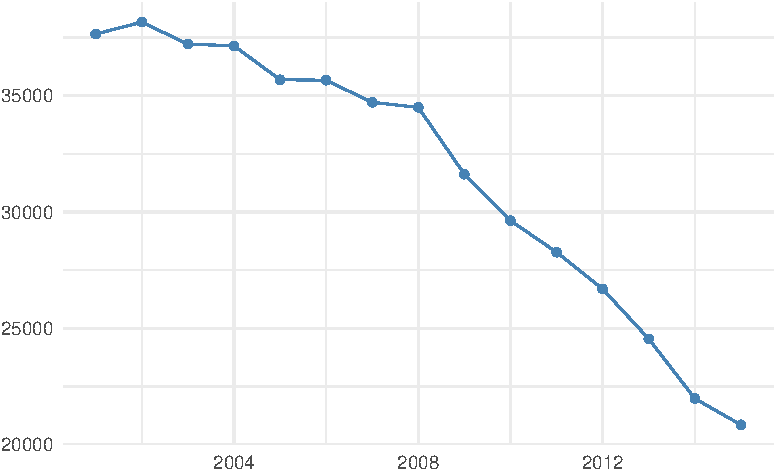
\includegraphics{201081646_MATH5741M_files/figure-latex/fig-1} 

}

\caption{Crimes evolution 2001-2015}\label{fig:fig}
\end{figure}

Figure 2 depicts the annual frequency of crimes per type and their
trend. The most common types of crime are Theft and Batery. All types
have been falling to a greater or lesser extent.

\begin{figure}[H]

{\centering 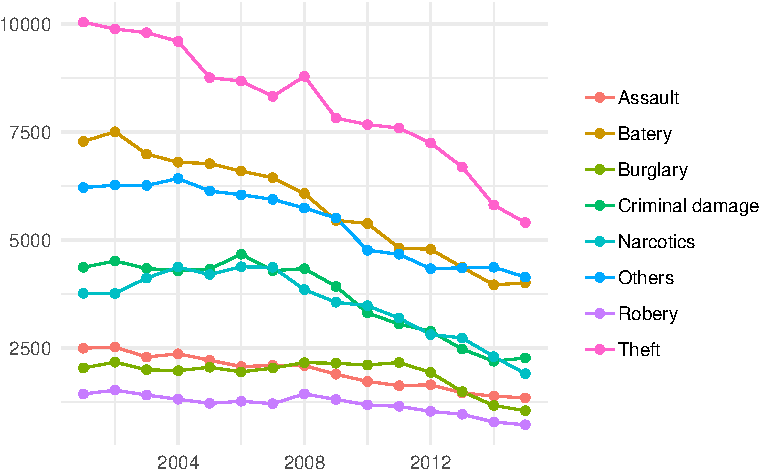
\includegraphics{201081646_MATH5741M_files/figure-latex/fig2-1} 

}

\caption{Crimes evolution per type of crime 2001-2015}\label{fig:fig2}
\end{figure}

\pagebreak

\subsubsection{What time of day do most crime
occur?}\label{what-time-of-day-do-most-crime-occur}

The following bar graph (Figure 3) shows the number of crimes increases
gradually from 05:00 in the morning (the hour with less crimes) until
20:00 in the evening (the hour with the most crimes). The hours of 12:00
and 00:00 are exceptionally high, at a similar level as 20:00.

\begin{figure}[H]

{\centering 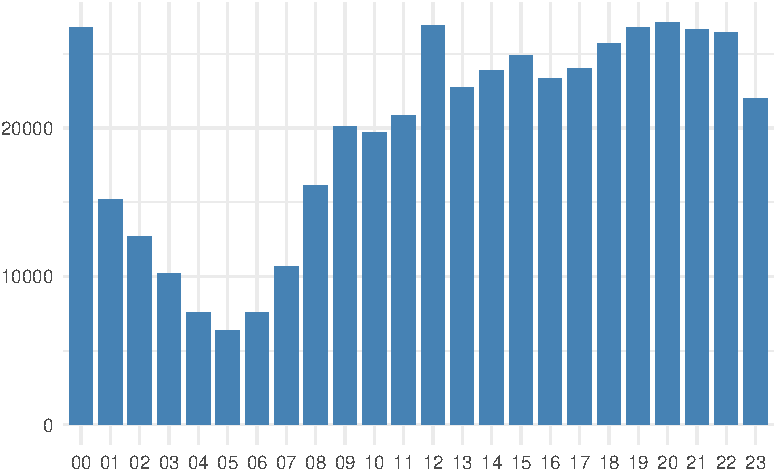
\includegraphics{201081646_MATH5741M_files/figure-latex/fig3-1} 

}

\caption{Crimes per hour}\label{fig:fig3}
\end{figure}

The heat-map in Figure 4 shows the distribution of number of crimes per
hour and type. For example, we can see that the peak hours of Theft and
Others are at 00:00, 09:00 and 12:00. Narcotics concentrate between
10:00 to 14:00 and 19:00 to 22:00. Other types are more evenly
distributed throughout the day.

\begin{figure}[H]

{\centering 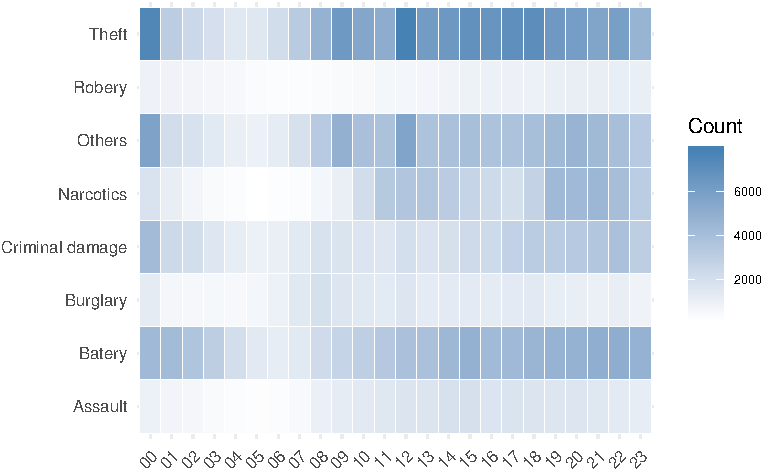
\includegraphics{201081646_MATH5741M_files/figure-latex/fig4-1} 

}

\caption{Type of crime vs hour}\label{fig:fig4}
\end{figure}

\pagebreak

\subsubsection{In which locations of the city is crime more likely to
happen?}\label{in-which-locations-of-the-city-is-crime-more-likely-to-happen}

As is illustrated by Figure 5, most crimes happen in the street,
followed by Residences and Apartments.

\begin{figure}[H]

{\centering 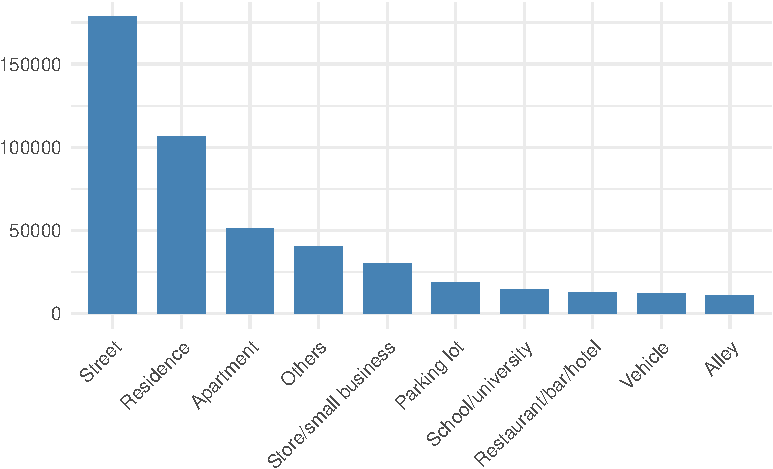
\includegraphics{201081646_MATH5741M_files/figure-latex/fig5-1} 

}

\caption{Crimes per location}\label{fig:fig5}
\end{figure}

If we visualise the distribution of crimes per location and type (Figure
6), we can see that some types occur in specific locations. For
instance, Robery is recorded almost enterily in the Street, as well as
Narcotics. However, Burglary and Others are registered particularly in
Reseidences or Apartments. What makes sense.

\begin{figure}[H]

{\centering 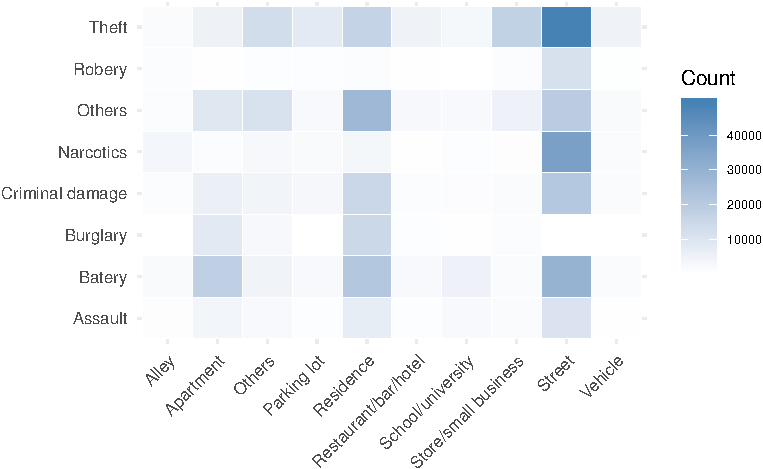
\includegraphics{201081646_MATH5741M_files/figure-latex/fig6-1} 

}

\caption{Type of crime vs location}\label{fig:fig6}
\end{figure}

\pagebreak

\subsubsection{Which districts are more potentially
dangerous?}\label{which-districts-are-more-potentially-dangerous}

Finally, in Figure 7, we visualise the number of crimes per districts.
The most dangerous district seems number 8, with more than 30,000
records in the 15 years, while district 20 with less than 10,000 seems
the safest.

\begin{figure}[htbp]
\centering
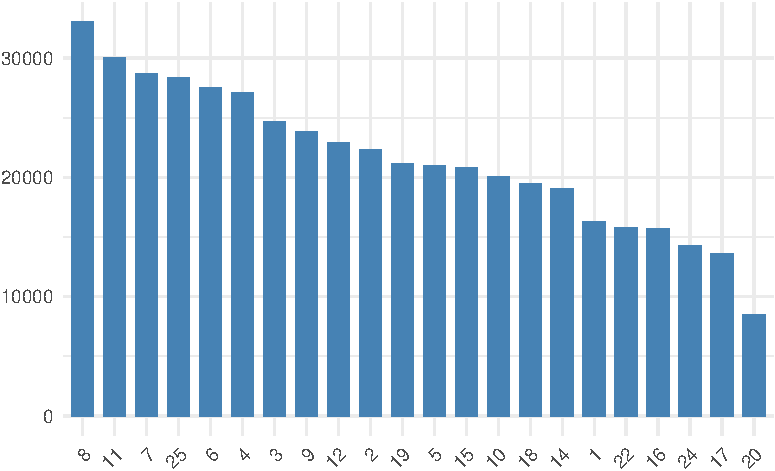
\includegraphics{201081646_MATH5741M_files/figure-latex/fig7-1.pdf}
\caption{Crimes per district}
\end{figure}

Figure 8 ilustrates some interesting findings in the relations between
the type of crime and districts where they occurred. For example, we can
see that districts 1, 8, 12 and 18 are particularly dangerous in terms
of Theft, that districts 7 and 11 stand out in terms of Batery, but
above all that Narcotics crime concentrates in district 11 and 15.

\begin{figure}[H]

{\centering 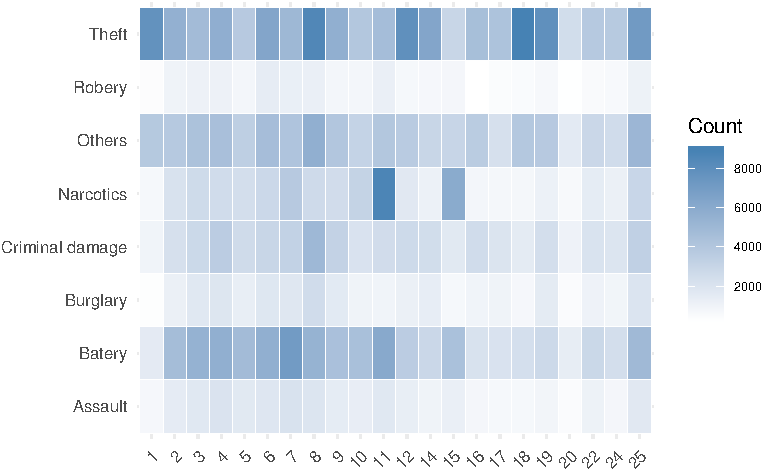
\includegraphics{201081646_MATH5741M_files/figure-latex/fig8-1} 

}

\caption{Type of crime vs district}\label{fig:fig8}
\end{figure}


\end{document}
